\documentclass[ignorenonframetext,]{beamer}

\usetheme{frankfurt}

\usepackage{amssymb,amsmath}
\usepackage{ifxetex,ifluatex}
\usepackage{fixltx2e} % provides \textsubscript
\usepackage{lmodern}
\ifxetex
\usepackage{fontspec,xltxtra,xunicode}
\defaultfontfeatures{Mapping=tex-text,Scale=MatchLowercase}
\newcommand{\euro}{€}
\else
\ifluatex
\usepackage{fontspec}
\defaultfontfeatures{Mapping=tex-text,Scale=MatchLowercase}
\newcommand{\euro}{€}
\else
\usepackage[T1]{fontenc}
\usepackage[utf8]{inputenc}
\fi
\fi
% use upquote if available, for straight quotes in verbatim environments
\IfFileExists{upquote.sty}{\usepackage{upquote}}{}
% use microtype if available
\IfFileExists{microtype.sty}{\usepackage{microtype}}{}



\usepackage{graphicx}
\makeatletter
\def\maxwidth{\ifdim\Gin@nat@width>\linewidth\linewidth\else\Gin@nat@width\fi}
\def\maxheight{\ifdim\Gin@nat@height>\textheight0.8\textheight\else\Gin@nat@height\fi}
\makeatother
% Scale images if necessary, so that they will not overflow the page
% margins by default, and it is still possible to overwrite the defaults
% using explicit options in \includegraphics[width, height, ...]{}
\setkeys{Gin}{width=\maxwidth,height=\maxheight,keepaspectratio}

\providecommand{\tightlist}{%
	\setlength{\itemsep}{0pt}\setlength{\parskip}{0pt}}
\setcounter{secnumdepth}{5}

\setlength{\parindent}{0pt}
\setlength{\parskip}{6pt plus 2pt minus 1pt}
\setlength{\emergencystretch}{3em}  % prevent overfull lines
\setcounter{secnumdepth}{0}


\usepackage{graphicx}
%\setbeamertemplate{caption}[numbered]
\usepackage[]{hyperref}
\hypersetup{linkcolor=black}
\urlstyle{same}  % don't use monospace font for urls
%\mode<presentation>
%\usepackage{amsmath}
\usepackage{tcolorbox}
\usepackage{multicol}

\usepackage{color}
\usepackage{float}

\definecolor{negro}{RGB}{0, 0, 0}
\definecolor{verdetelecomclaro}{RGB}{251, 255, 172}
\definecolor{iosOrange}{HTML}{FF9500}
\definecolor{iosGreen}{HTML}{4cd964}
\definecolor{iosRed}{HTML}{FF3B30}
\definecolor{iosPink}{HTML}{FF2D55}
\definecolor{iosBlue}{HTML}{007AFF}
\definecolor{iosLBlue}{HTML}{34AADC}

\newfontfamily{\sectionsfont}[Path = ./fonts/,
Extension = .ttf,
UprightFont = *-Regular,
ItalicFont = *-Italic,
BoldFont = *-Bold]{NotoSerif}

\setbeamertemplate{navigation symbols}{}
\setbeamertemplate{title page}[empty]

\setbeamerfont{frametitle}{family=\bfseries\sectionsfont}
\setbeamerfont{title}{family=\sectionsfont}



\setbeamerfont{subtitle}{size=\small}

\setbeamertemplate{itemize items}[square]

\setbeamercovered{transparent}

\setbeamercolor{block title}{bg=iosBlue!30,fg=black}
%\setbeamercolor{title}{bg=iosBlue!30, fg = red}
\setbeamercolor{title}{bg=iosBlue!50!white,fg=black}
\setbeamercolor{frametitle}{fg=iosBlue,bg=iosLBlue!5!white}
\setbeamercolor{section in head/foot}{fg=iosLBlue,bg=iosLBlue!5!white}
%\setbeamercolor{structure}{fg=iosRed}
%\setbeamercolor{structure}{fg=iosRed}
\setbeamercolor{item projected}{bg=iosBlue}
\setbeamercolor{itemize item}{fg=iosBlue}
\setbeamercolor{section in toc}{fg=black}

\setsansfont[Mapping=tex-text,
Path = ./fonts/,
Extension = .ttf,
ItalicFont = *-Italic,
UprightFont = *-Regular,
BoldItalicFont = *-BoldItalic,
BoldFont = *-Bold]{NotoSans}

\setmonofont[Path = ./fonts/,
Extension = .ttf,
UprightFont = *-Regular,
BoldFont = *-Black]{Inconsolata}

\newtcolorbox{box_naranja}{enhanced,sharp corners,colback=iosOrange!20!white,colframe=iosOrange}
\newtcolorbox{box_verde}[1]{rightrule=0pt,toprule=0pt, leftrule=0pt,bottomrule=1pt,colback=iosGreen!5!white,colframe=iosGreen!80!black,fonttitle=\sffamily,title=#1}
\newtcolorbox{box_rosa}[1]{enhanced,sharp corners,drop fuzzy shadow,rightrule=0pt,toprule=0pt, leftrule=0pt,bottomrule=0pt,colback=iosPink!5!white,colframe=iosPink!95!black,fonttitle=\sffamily,title=#1}
\newtcolorbox{box_roja}[1]{enhanced,sharp corners,drop fuzzy shadow,rightrule=0pt,toprule=0pt, leftrule=0pt,bottomrule=2pt,colback=iosRed!5!white,colframe=iosRed!80!black,fonttitle=\sffamily,title=#1}
\newtcolorbox{box_azul}[1]{enhanced,sharp corners, drop fuzzy shadow,rightrule=0pt,toprule=0pt, leftrule=0pt,bottomrule=1pt,colback=iosLBlue!5!white, colframe=iosLBlue!80!black,colbacktitle=iosLBlue!80!black,fonttitle=\sffamily,title=#1}

\usepackage{listings}
\lstdefinestyle{codechunk}{
	backgroundcolor=\color[HTML]{daf1f5},
	language=R,
	showstringspaces=false,
	basicstyle=\footnotesize\ttfamily,
	keywordstyle=\bfseries\color[HTML]{90323D},
	keywordstyle={[2]\color[HTML]{5CB22E}},
	keywords=[2]{TRUE,FALSE},
	stringstyle=\color[HTML]{EBA433},
	alsoletter ={_},
	otherkeywords={ggplot,geom_ridges,stat_summary,aes,_qq,_line,facet_wrap,fct_reorder,gg,filter,group_by,mutate,quantiles,gg_rf,gg_pt,_sl,bootstrap_anova,summarise,map_int,pivot_longer,seq_along,geom_boxplot,geom_point,geom_hline,geom_vline,stat_smooth,select,geom_jitter,pull,map,tibble,geom_density_ridges,crossing,geom_line,geom_,as.Date,as_tibble,ungroup,kable,pivot_wider,bind_rows,ggAcf,theme,ylab,xlab,sscale_fill_continuous,arrange,unnest_wider},
	deletekeywords={col,R,names,data,colors,args,residuals,null,_}}
\lstset{escapechar=\&}
\lstdefinestyle{output}{
	backgroundcolor=\color[HTML]{FCFFF7},
	language=R,
	basicstyle=\ttfamily}

\AtBeginPart{}
\AtBeginSection{}
\AtBeginSubsection{}
\AtBeginSubsubsection{}
\setlength{\emergencystretch}{0em}
\setlength{\parskip}{0pt}

\title{\textbf{Menos for, más purrr}:\\
Programación funcional con R}
\author{Nacho Evangelista}
\date{18 de febrero de 2020}

\begin{document}
		\frame{\titlepage}
		
		\begin{frame}
\frametitle{Contenido} % Table of contents slide, comment this block out to remove it
\setbeamertemplate{sections/subsections in toc}[square]
\begin{columns}[t]
	\column{.5\textwidth}
		\tableofcontents[sections={1-3}]
	\column{.5\textwidth}
		\tableofcontents[sections={4-8}]
\end{columns}
%\tableofcontents % Throughout your presentation, if you choose to use \section{} and \subsection{} commands, these will automatically be printed on this slide as an overview of your presentation
\end{frame}

\hypertarget{introducciuxf3n}{%
\section{Introducción}\label{introducciuxf3n}}

\hypertarget{motivaciuxf3n}{%
\subsection{Motivación}\label{motivaciuxf3n}}

\begin{frame}{A}
\protect\hypertarget{a}{}
\begin{itemize}
\tightlist
\item
  Bullet 1: holis
\item
  Bullet 2
\item
  Bullet 3
\end{itemize}
\end{frame}

\hypertarget{listas-en-r}{%
\subsection{Listas en R}\label{listas-en-r}}

\begin{frame}{A}
\protect\hypertarget{a-1}{}
\end{frame}

\hypertarget{purrr}{%
\section{purrr}\label{purrr}}

\hypertarget{la-funciuxf3n}{%
\subsection{\texorpdfstring{La función
\texttt{map}}{La función }}\label{la-funciuxf3n}}

\begin{frame}[fragile]{A}
\protect\hypertarget{a-2}{}
\begin{lstlisting}[style=codechunk]
summary(cars)
\end{lstlisting}

\begin{verbatim}
##      speed           dist       
##  Min.   : 4.0   Min.   :  2.00  
##  1st Qu.:12.0   1st Qu.: 26.00  
##  Median :15.0   Median : 36.00  
##  Mean   :15.4   Mean   : 42.98  
##  3rd Qu.:19.0   3rd Qu.: 56.00  
##  Max.   :25.0   Max.   :120.00
\end{verbatim}
\end{frame}

\hypertarget{acomodando-el-tipo-de-salida}{%
\subsection{Acomodando el tipo de
salida}\label{acomodando-el-tipo-de-salida}}

\begin{frame}{A}
\protect\hypertarget{a-3}{}
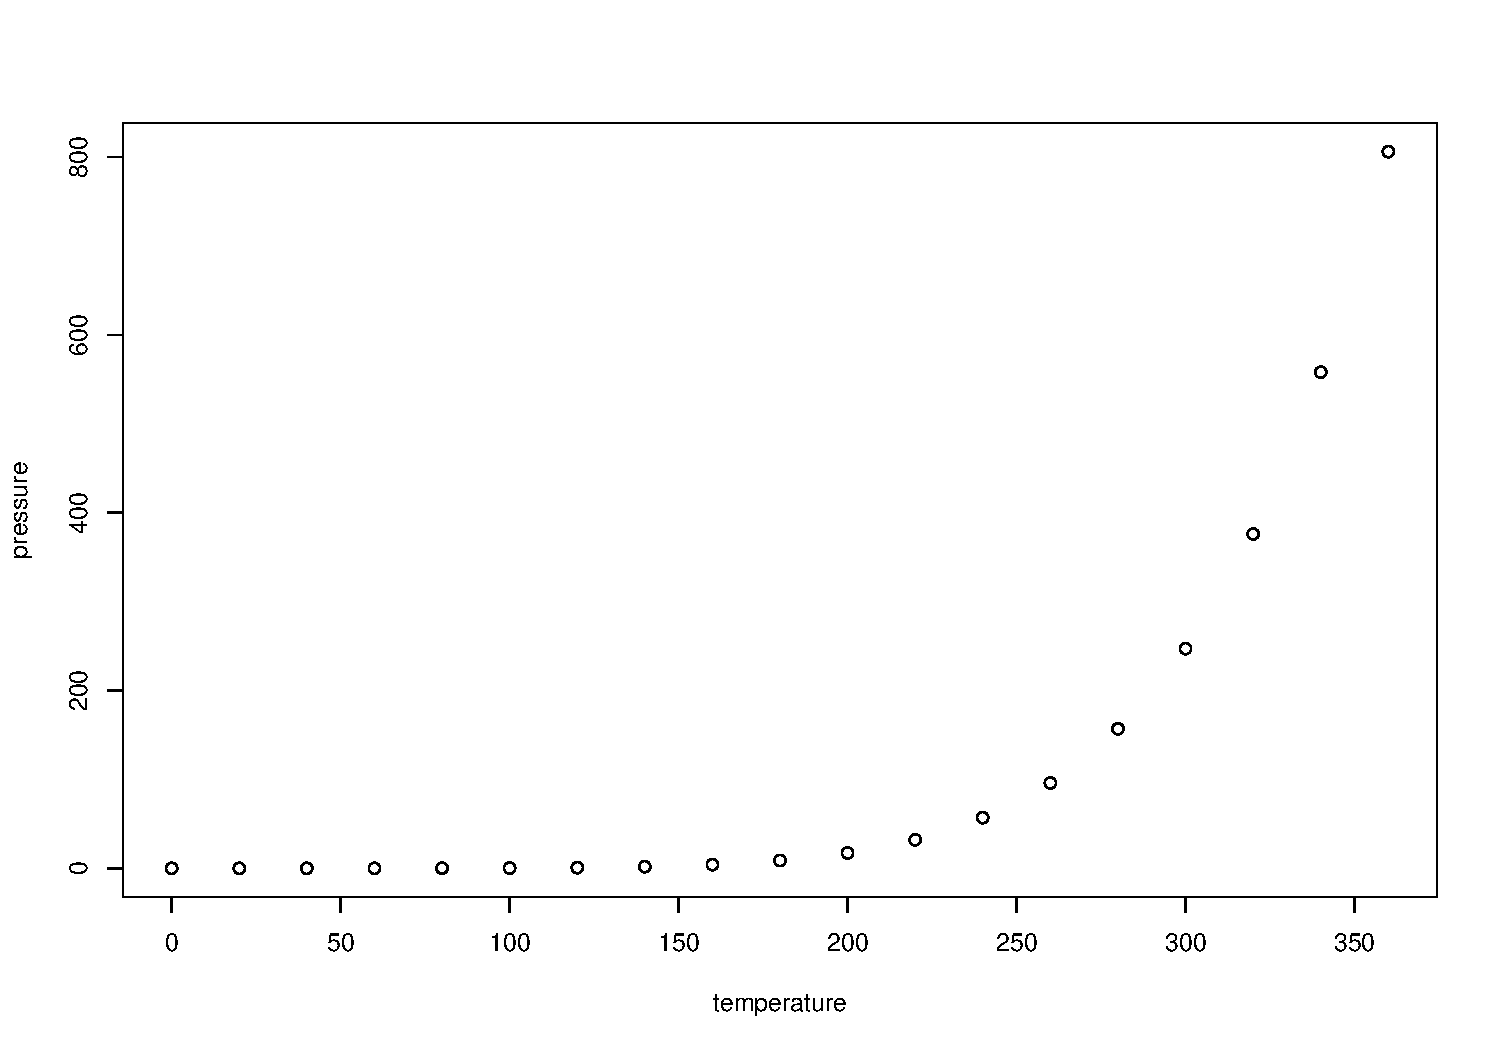
\includegraphics{Purrr_files/figure-beamer/pressure-1.pdf}
\end{frame}

\hypertarget{funciones-anuxf3nimas}{%
\subsection{Funciones anónimas}\label{funciones-anuxf3nimas}}

\begin{frame}{A}
\protect\hypertarget{a-4}{}
\end{frame}

\hypertarget{muxfaltiples-argumentos}{%
\subsection{Múltiples argumentos}\label{muxfaltiples-argumentos}}

\begin{frame}{\texttt{map2}}
\protect\hypertarget{section}{}
\end{frame}

\hypertarget{dataframes}{%
\subsection{dataframes}\label{dataframes}}

\begin{frame}{Pero yo nunca usé listas\ldots{}}
\protect\hypertarget{pero-yo-nunca-usuxe9-listas}{}
\end{frame}

\hypertarget{purrr-tidyr-dplyr}{%
\section{purrr + tidyr + dplyr}\label{purrr-tidyr-dplyr}}

\hypertarget{section-1}{%
\subsection{\texorpdfstring{\texttt{mutate} +
\texttt{purrr}}{ + }}\label{section-1}}

\hypertarget{columnas-lista-y-dataframes-anidados}{%
\subsection{Columnas lista y dataframes
anidados}\label{columnas-lista-y-dataframes-anidados}}

\begin{frame}{¿Cómo se construyen?}
\protect\hypertarget{cuxf3mo-se-construyen}{}
\begin{itemize}
\tightlist
\item
  Definición:
\item
  Usando \texttt{nest}
\end{itemize}
\end{frame}

\begin{frame}{¿Por qué necesito purrr?}
\protect\hypertarget{por-quuxe9-necesito-purrr}{}
\end{frame}

\hypertarget{ejemplos}{%
\subsection{Ejemplos}\label{ejemplos}}

\begin{frame}{Secuencia de fechas}
\protect\hypertarget{secuencia-de-fechas}{}
\end{frame}

\begin{frame}{Coeficiente de correlación}
\protect\hypertarget{coeficiente-de-correlaciuxf3n}{}
\end{frame}

\begin{frame}{Abrir varios archivos a la vez}
\protect\hypertarget{abrir-varios-archivos-a-la-vez}{}
\end{frame}

\begin{frame}{Rotar puntos}
\protect\hypertarget{rotar-puntos}{}
\end{frame}

\begin{frame}{Train/test}
\protect\hypertarget{traintest}{}
\end{frame}

\begin{frame}{Múltiples plots}
\protect\hypertarget{muxfaltiples-plots}{}
\end{frame}

\hypertarget{extra}{%
\section{Extra}\label{extra}}

\hypertarget{puede-fallar}{%
\subsection{Puede fallar\ldots{}}\label{puede-fallar}}

\begin{frame}{\texttt{possibly}}
\protect\hypertarget{section-2}{}
\end{frame}

\hypertarget{section-3}{%
\subsection{\texorpdfstring{\texttt{repeat}}{}}\label{section-3}}

\hypertarget{resumen}{%
\section{Resumen}\label{resumen}}

\begin{frame}{Resumen}
\protect\hypertarget{resumen-1}{}
\end{frame}

\end{document}